\documentclass[11pt]{article}
\usepackage[includeheadfoot, top=1.0in, bottom=1.0in, hmargin=1.0in]{geometry}
\usepackage[utf8]{inputenc}
\usepackage{fancyhdr}
\usepackage{url}
\pagestyle{fancy}
\usepackage{setspace}
\usepackage{tabularx}
\usepackage{graphicx}
\usepackage{caption}
\usepackage{subcaption}
\usepackage{hyperref}
\usepackage{multicol}
\usepackage{amsmath}
\usepackage{amssymb}
\usepackage{enumitem}
\usepackage{array}
\usepackage{xcolor}

\lhead{Astronomy Lab I --- \textbf{Answer Key}}
\rhead{Fall 2026}
\cfoot{\thepage}

% --- helpers ---------------------------------------------------------
\newenvironment{choices}
  {\begin{list}{}{%
     \setlength{\leftmargin}{2em}\setlength{\itemsep}{2pt}%
     \setlength{\topsep}{4pt}\setlength{\parsep}{0pt}}}
  {\end{list}}
\newcommand{\ch}[1]{\item[\textbf{(#1)}]}

\newcommand{\activity}[1]{%
  \par\smallskip\noindent
  \fbox{\parbox{0.965\textwidth}{\small #1}}\par\smallskip}

\newcommand{\card}[2]{%
  \par\medskip\noindent
  \fbox{\parbox{0.94\textwidth}{%
    \textbf{#1}\par\smallskip #2\par\smallskip
 }}}

% point-value tag, printed at the start of a question or part
\newcommand{\pts}[1]{\textit{[#1 points]}\ }

\setlist[enumerate]{itemsep=11pt, topsep=6pt}

% answer block
\newcommand{\ans}[1]{%
  \par\smallskip\noindent{\color{blue!55!black}\textbf{Answer:}}\ #1\par\smallskip}
\newcommand{\note}[1]{%
  \par\noindent{\color{red!55!black}\textbf{Note:}}\ #1\par}

\begin{document}

\begin{center}
\huge{Lab 5: Pseudoscience}\\[4pt]
\Large\textbf{Answer Key}
\end{center}

\bigskip
\noindent\textit{``Anti-intellectualism has been a constant thread winding its
way through our political and cultural life, nurtured by the false notion
that democracy means that `my ignorance is just as good as your
knowledge.'''} --- Isaac Asimov

%%%%%%%%%%%%%%%%%%%%%%% INTRO %%%%%%%%%%%%%%%%%%%%%%%
\section{Introduction}
What is science? What is pseudoscience? As you navigate today's world, rife with claims stemming from junk science (or no science at all), it is important to be able to discern between the two. In today's lab, we will give you the qualitative tools to make the distinction between science and pseudoscience. We will also disprove some pseudo-scientific theories, using probabilities and geometry.

%%%%%%%%%%%%%%%%%%%%%%%
\section{What Makes Something Scientific?}
\label{sec:what_makes_something_scientific}
A theory, model, prediction, measurement, or observation is generally
considered \textbf{scientific} if it is:
\begin{enumerate}[label=(\alph*)]
    \item \textbf{Repeatable} (at least in principle, as may be the case with rare events we cannot control)
    \item \textbf{Objective}
    \item \textbf{Predictive}
    \item \textbf{Falsifiable}
\end{enumerate}
\begin{enumerate}
    \item \pts{4} Briefly, what do each of these four words mean to you? Discuss with your group, and write down your answers.

    \ans{1 point for each word explained. Answers just need to get the gist of it:
    \\
    \textbf{Repeatable:} an experiment can be done over and over again, and always give you the same result. \\
    
    \textbf{Objective:} Outcome doesn't change depending on who/what does it \\
    
    \textbf{Predictive:} there's an idea of what will
    happen before it happens. \\
    
    \textbf{Falsifiable:} there exists a possible observation that
    would prove the claim wrong}


\end{enumerate}

What constitutes a scientific theory? A theory is an explanation of some aspect of the natural world that has been repeatedly upheld by rigorous experiment and never falsified. Theories begin as hypotheses: testable predictions that can be corroborated or falsified via the scientific method. Theories are similar to scientific laws, but are usually broader in scope (their explanatory power extends further). For instance, Kepler's First Law states that the orbit of every planet is an ellipse with the Sun at one focus. Clearly, this describes a specific phenomenon, in contrast to, for instance, the Theory of General Relativity, which explains all phenomena associated with gravitation. Both laws and theories are scientific fact. One common misconception is that scientific theories are ``just theories'': that they have yet to become scientific law, or that they are on equal footing with one or more alternative ideas.

%%%%%%%%%%%%%%%%%%%%%%%
\section{Pseudoscience}
\textit{Pseudoscience} refers to any belief, claim, or practice that is
presented as scientific but does not actually follow the scientific method
or possess the characteristics described in Section \ref{sec:what_makes_something_scientific}. Pseudoscience often uses the language or
appearance of science without following the standards that make a claim
scientifically testable. Examples of pseudoscience range from the fairly harmless
(cryptozoology -- the belief that creatures like the Loch Ness monster
exist) to the actively dangerous (medical pseudoscience that leads people to
forgo real treatment) to the historically horrific (``scientific racism,''
the discredited claim that some races are biologically superior to others).
It is also important to distinguish between a claim that is wrong, a claim that has not been tested, and a claim that is presented as scientific but does not actually allow itself to be tested. Plenty of real science turns out to be wrong. And ``not yet tested'' is
a \emph{status}: an untested claim is one somebody
could go and check tomorrow. A pseudoscientific claim is one where attempting to verify it reveals that it is incompatible with the scientific method at all.

%%%%%%%%%%%%%%%%%%%%%%%
\section{Evaluating Scientific Claims}
Let's practice using the above 4  criteria on some claims. Scientists must think critically about  the information they consume, whether it is found on Instagram reels or in a paper on the arxiv.
Below are three claims, in no particular order.
\begin{center}
\begin{tabular}{@{}p{0.06\textwidth}p{0.85\textwidth}@{}}
\textbf{A1.} & Mercury is in retrograde, so you should avoid signing
contracts this week. \\[6pt]
\textbf{A2.} & People who sleep less than six hours a night are more likely
to report symptoms of depression. \\[6pt]
\textbf{A3.} & People who drink coffee live longer.
\end{tabular}
\end{center}
\begin{enumerate}
    \setcounter{enumi}{1}
    \item Let's evaluate claim \textbf{A1} using the criteria from Section 2.
    \begin{enumerate}[label=(\alph*)]
        \item \pts{1} What observation or result, if any, would convince you that this claim
        is \emph{false}?  Consider the non-committal language: "should avoid".

        \ans{Nothing. The way A1 is phrased means it can be waved off as a fluke if someone signs a contract during Mercury retrograde, and it goes well.}
        
        \item \pts{2} Would you classify this claim as \textbf{scientifically
        testable}, \textbf{pseudoscientific}, or \textbf{not yet tested}?
        From the four criteria in Section 2, choose \textit{one} and explain why it cannot be met.

        \ans{Pseudoscientific. It isn't objective (a ``bad'' outcome is subjective), it isn't  predictive (it doesn't say anything about the type of
    contract or how much risk to expect etc.), and it isn't
    falsifiable (any bad outcome ``confirms'' it, any good outcome can be
    explained away - this relates to the previous part).}


        \item \pts{1} Suppose astrology has no real effect on how contracts turn out.
        Why might someone still be convinced, from their own experience, that the
        advice works? 
        
        \ans{One point each for anything reasonable. Examples: \\
        - If you've been told a week is risky, you will notice and
        remember the mishaps more than anything that went fine (confirmation
        bias). \\
        - ``Goes wrong'' is vague enough that almost any week qualifies. \\
        - If you think the week will go badly, you may unknowingly rush, 
        or second-guess decisions and get a worse outcome. A
        self-fulfilling prophecy!  \\
        - If you've got friends who really believe in astrology, they might
        reinforce the belief. \\
        }
    \end{enumerate}
\end{enumerate}


It is tempting to jump from a correlation straight to cause and effect: since Y followed X, X \textit{must} have caused it. However, correlation doesn't prove causation. X might cause Y, Y might cause X, or a hidden third factor could be driving both, or it could simply be a coincidence. While correlations are great for sparking curiosity and guiding further research, we must be careful not to treat them as anything more.
\begin{enumerate}
\setcounter{enumi}{2}
    \item \pts{2} Claims \textbf{A2} and \textbf{A3} are both based on correlations found in real data. For each, give one possible explanation other than ``X causes Y.''

    \ans{1 point each for a reasonable alternative explanation.\\
    \textbf{A2 (sleep/depression):} depression itself disrupts sleep.  An external factor like stress or illness can drive both
    short sleep and low mood. \\
    \textbf{A3 (coffee/longevity):} Someone healthy enough to make it to old age would have more time to drink more coffee (or something like that). People who drink coffee may have higher incomes (coffee is more expensive than tea), or be more active, or be more social, which can increase longevity.}
\end{enumerate}
        


%%%%%%%%%%%%%%%%%%%%%%% IN THE WILD %%%%%%%%%%%%%%%%%%%%%%%

\section{Evaluating an Argument}

Let's look at a confident, AI-generated (because this is the world we live in) argument, where it takes a little more discernment to evaluate its credibility. The questions below help us evaluate how well a particular argument is actually constructed.


\card{}{%
``Hospital emergency rooms and police stations consistently report a dramatic surge in psychiatric admissions, violent crimes, and trauma cases during the full moon. Because the human body is composed of roughly 60\% water, the Moon's gravitational pull exerts a tidal force on human brain tissue and bodily fluids in the exact same way it creates ocean tides. This monthly gravitational stress disrupts neurological activity and sleep cycles, directly causing heightened aggression and erratic behavior across human populations during full lunar phases.''}

\begin{enumerate}
    \setcounter{enumi}{3}
    \item Answer the following questions in 1-2 sentences each:
    \begin{enumerate}[label=(\alph*)]

    \item \pts{1} The argument asserts that emergency rooms and police stations ``consistently report a dramatic surge'' during full moons. Before trying to explain \emph{why} this happens, what step must a scientist take regarding this initial premise?

\ans{A scientist must first check whether the claimed effect actually exists in empirical data (i.e., check if the premise is true). }


        \item \pts{1} The author claims that lunar gravity exerts a "tidal force on human brain tissue" because humans are made of water. What is flawed about this  argument? 
        
        \ans{Tidal forces depend on the size of the object across which gravity acts. Humans are very tiny compared to the ocean, so it has a very negligible effect on us.}


        \item \pts{1} The argument claims that full moons cause increased
        aggression and erratic behavior. Give one possible alternative
        explanation for the claimed pattern.
        
        \ans{1 point for identifying relevant evidence, 1 point for a reasonable
        alternative explanation, and 1 point for explaining how the evidence
        could distinguish between them. Examples of alternative explanations
        include coincidence, differences in reporting behavior, or other factors
        that happen to coincide with full moons.}

        
    \end{enumerate}
\end{enumerate}

%%%%%%%%%%%%%%%%%%%%%%% HOROSCOPES %%%%%%%%%%%%%%%%%%%%%%%
\section{Astrology \& the Binomial Distribution}

Astrology proposes that the position of celestial objects (e.g. the sun, moon, and planets) influences terrestial events. It is rooted in ancient practices from all over the globe, with signs of it being practiced from the 2nd millenium BCE! It's a very human desire to understand why certain events happen (good or bad), and it's remarkable how well-studied the night sky became because of it. Indeed, there was almost no distinction between astrology and astronomy until the late Middle Ages.

\begin{figure}
    \centering
    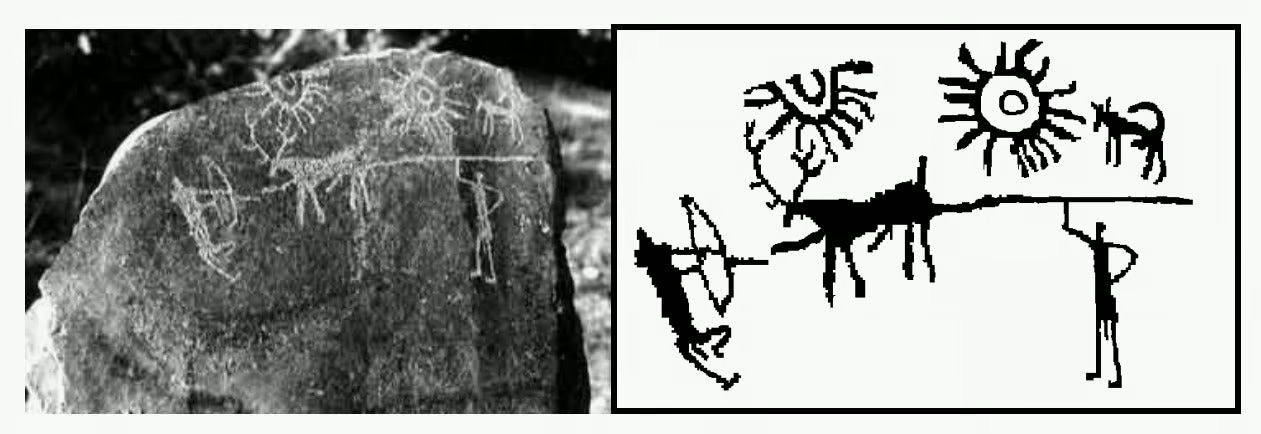
\includegraphics[width=0.75\linewidth]{ancient_sne.jpeg}
    \caption{Rock art dated to roughly 2100 BCE, that some astronomers believe depict the supernova HB9. Source: Quartz.com}
\end{figure}

These days, we may be exposed to astrology through social media or apps that generate \textbf{horoscopes}: regular predictions aligned with ones astrological natal chart. These horoscopes give
advice like ``do something that scares you today'' or ``avoid making
decisions about your living situation.'' Horoscopes are fun to check, but it is language that could arguably apply to anyone \footnote{This is such a common cognitive bias, that it has a name: the Barnum effect.}.


Let's check horoscopes for the Sun signs from three different sources (see handout), where the signs have been stripped off. From each of the three sources, pick the one that best matches your week so far. Once everyone has chosen, we'll
reveal the actual signs and see how you did.
For reference:
\begin{center}
\begin{tabular}{@{}ll@{}}
Aries: Mar 21 -- Apr 19 & Libra: Sep 23 -- Oct 22 \\
Taurus: Apr 20 -- May 20 & Scorpio: Oct 23 -- Nov 21 \\
Gemini: May 21 -- Jun 20 & Sagittarius: Nov 22 -- Dec 19 \\
Cancer: Jun 21 -- Jul 22 & Capricorn: Dec 22 -- Jan 19 \\
Leo: Jul 23 -- Aug 22 & Aquarius: Jan 20 -- Feb 18 \\
Virgo: Aug 23 -- Sep 22 & Pisces: Feb 19 -- Mar 20
\end{tabular}
\end{center}
\subsection{The Binomial Distribution}
If astrology worked, everyone would pick the horoscope matching their real
sign every time. If it doesn't work, that doesn't mean nobody ever picks
correctly -- pure chance will get some people right some of the time. If
the horoscope choices are unrelated to a person's actual sign, each choice
has a probability $p = 1/12$ of being correct. Treating the choices as
independent, the \textbf{binomial distribution} gives the probability of
getting exactly $k$ correct out of $n$ attempts:
\begin{equation}
    P(k \mid n, p) = \frac{n!}{k!\,(n-k)!}\, p^k (1-p)^{(n-k)}.
\end{equation}
\begin{enumerate}
    \setcounter{enumi}{4}
    \item \pts{3} What are $p$, $k$, and $n$ for our horoscope experiment?

    \ans{\textbf{$n=3$} is the number of horoscope sources each
    student picks from (one guess per source). \textbf{$p=1/12$ }is the probability
    of guessing any one correctly.
    $k$ is the number of correct guesses out of the 3 --- this varies!!!  }

    \item
    \pts{4} What is the probability of guessing zero, one, two, or three
        horoscopes correctly by pure chance?

    \ans{ \textbf{Probabilities
    (with $n=3$, $p=1/12$):} $P(0)=(11/12)^3\approx0.770$;
    $P(1)=3(1/12)(11/12)^2\approx0.210$; $P(2)=3(1/12)^2(11/12)\approx0.019$;
    $P(3)=(1/12)^3\approx0.0006$. (quick check: these four values should sum to
    $\approx1$}

   

        \item \pts{2} Plot the four results from above: $P(k \mid n, p)$ on the $y$-axis, $k$ on the $x$-axis. Label the axes.

        \ans{1 point for correct labels. 1 point for all 4 points.}

        \item \pts{3} How many did you get right? Take a few minutes to compare with your groupmates/classmates. Add their $k$-values to your plot, in a different symbol. Does the spread of correct guesses roughly follow
        the binomial distribution? 

        \ans{1 point for stating their $k$. 1 point for including their classmates values in the plot. 1 point for evaluating the spread.}

        \item \pts{1} Based on tonight's results, what do you conclude about the
        predictive power of horoscopes? 

        \ans{Not predictive (unless for some reason everyone guesses really well...}

\end{enumerate}

%%%%%%%%%%%%%%%%%%%%%%% FLAT EARTH %%%%%%%%%%%%%%%%%%%%%%%
\section{Flat Earth}

The Flat Earth theory is self-explanatory: it is the idea that the Earth is shaped like a flat plane, rather than a sphere. This claim is useful to examine because it makes a clear,
testable prediction: if the Earth is spherical, distant objects should
eventually disappear below the horizon. In this section you'll test that
prediction quantitatively, using two methods built on the same right
triangle.
\subsection{How Far Can You See?}
If the Earth were flat, you could see infinitely far, limited only by haze
and the resolving power of your eyes or telescope. On a spherical Earth,
the surface curves away from you and you are eventually limited by the
\textbf{horizon distance}.
For an observer at height $h$ above the surface of a sphere of radius $R$,
the distance to the horizon is

\begin{equation}
    d = \sqrt{2Rh + h^2} \approx \sqrt{2Rh}
\end{equation}

where the approximation holds when $h \ll R$. This is an application of
the Pythagorean theorem.

\begin{figure}
    \centering
    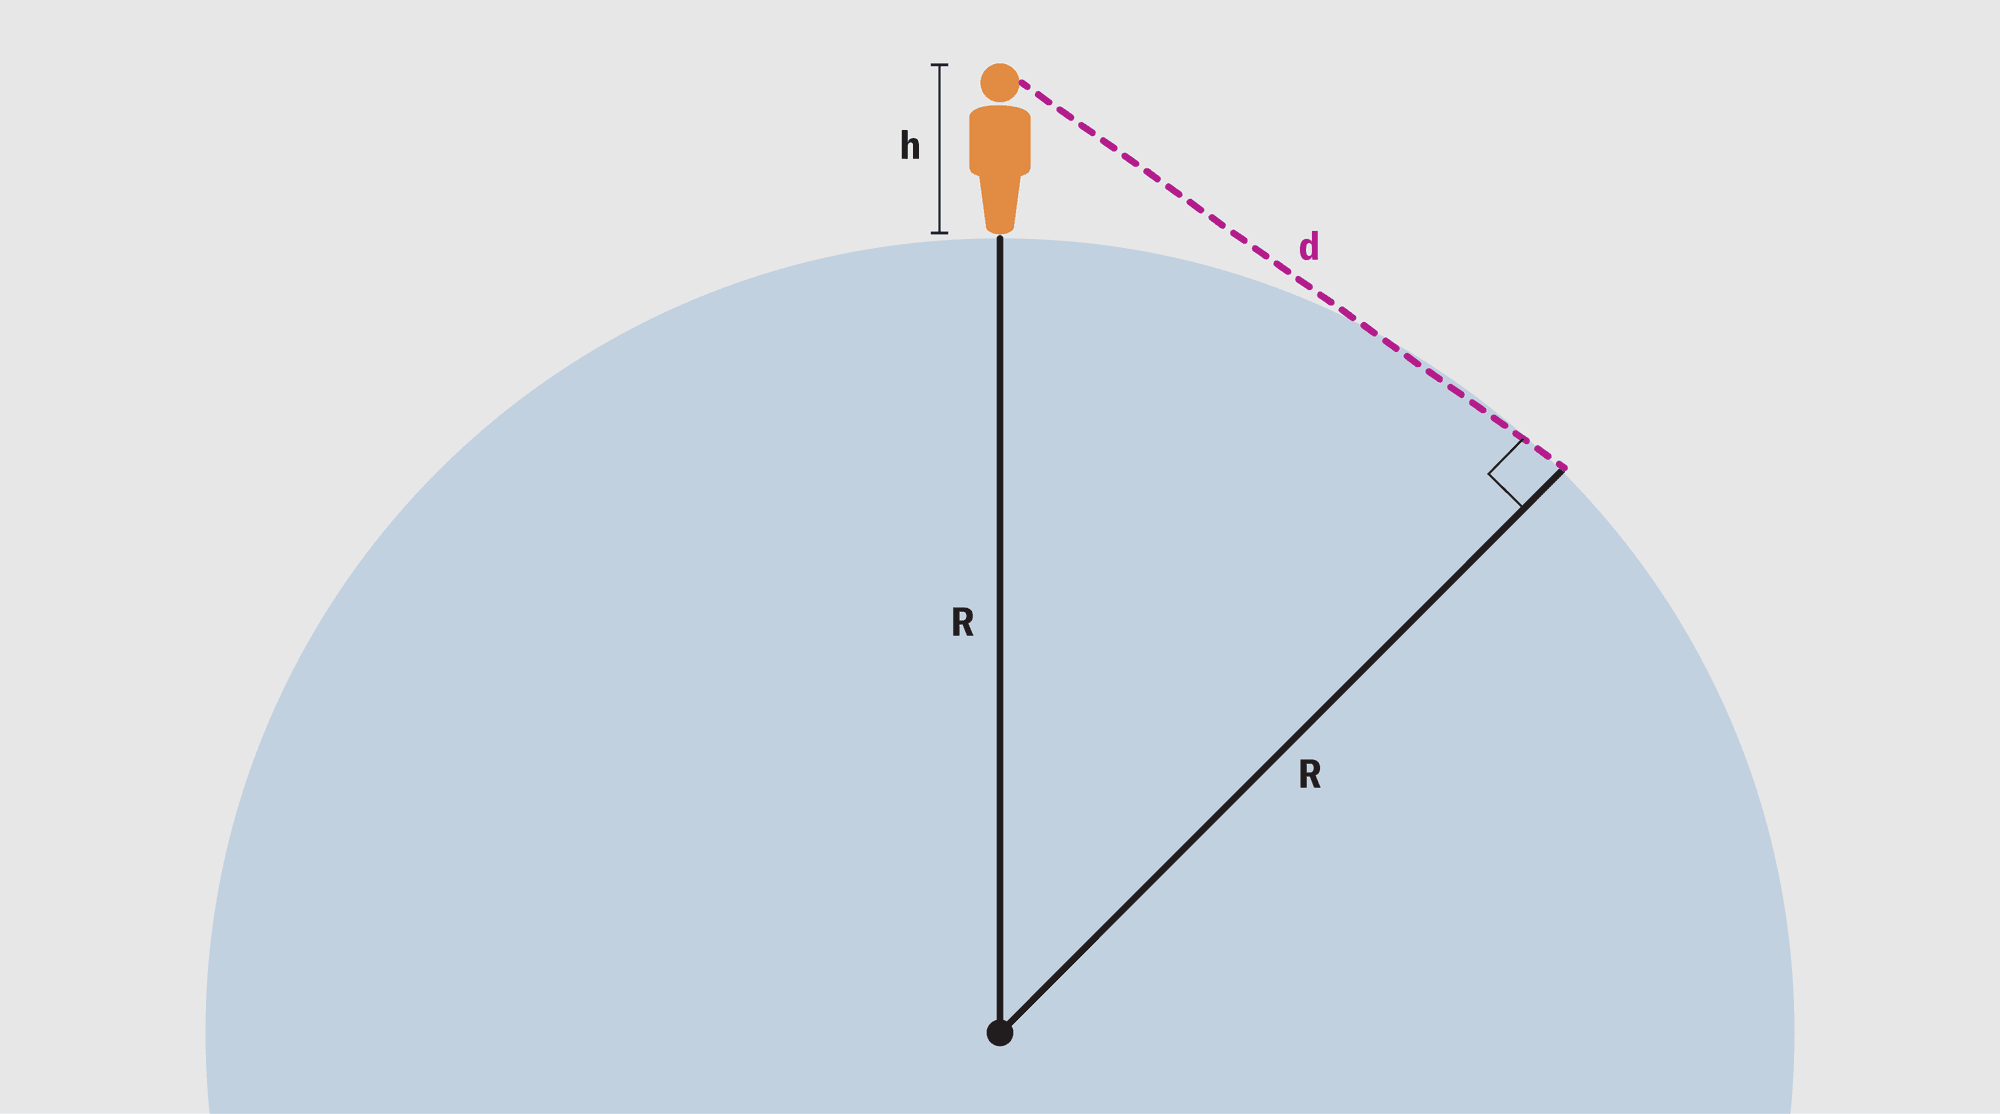
\includegraphics[width=0.5\linewidth]{horizon_distance.png}
    \caption{Visual of the horizon distance, $d$. Source: Scientific American}
    \label{fig:horizon_distance}
\end{figure}

\begin{enumerate}
    \setcounter{enumi}{9}
    \item The Earth's radius is 6{,}371~km. Be careful about units.
    \begin{enumerate}[label=(\alph*)]
        \item \pts{2} A person standing at the shore with their eyes 1.7~m above sea
        level can see how far to the horizon?

        \ans{\textbf{(a)} $h=1.7\text{ m}=0.0017\text{ km}$:
    $d=\sqrt{2(6371)(0.0017)}\text{ km}\approx\sqrt{21.66}\approx4.65$~km.}
    
        \item \pts{2} The Top of the Rock observation deck in Midtown Manhattan is
        about 260~m above sea level. How far can you see from there on a
        clear day?

        \ans{$h=260\text{ m}=0.260\text{ km}$:
    $d=\sqrt{2(6371)(0.260)}\text{ km}\approx\sqrt{3312.9}\approx57.5$~km.}

    
        \item \pts{2} If the Earth were flat, would either of those numbers exist at
        all? Explain.

        \ans{

    \textbf{(c)} No. On a flat Earth there is no geometric horizon.}
    \end{enumerate}

    


    \item \pts{3} Flat Earth proponents may point to photos or videos where a
    distant city skyline is visible across a lake as ``proof'' that there's
    no curvature. Using your horizon-distance formula, explain why tall
    buildings can remain visible well beyond the point where the shoreline
    itself has disappeared below the horizon.  \\ \textit{Hint: compare $h$ for the shoreline and for a tall building. What changes with $h$?}

    \ans{Horizon distance grows
with $\sqrt{h}$. The shoreline itself has
$h\approx 0$, so its own horizon distance is essentially zero: it
disappears from view almost immediately. A tall building has a much
larger $h$, so $d=\sqrt{2Rh}$ is correspondingly larger --- it stays
visible.}
\end{enumerate}

\subsection{Al-Biruni's Measurement}

Around 1020~CE, the Persian polymath Ab\=u Rayh\=an al-B\={\i}r\=un\={\i}
stood on a mountain near the Fort of Nandana, in what is now Punjab,
Pakistan. He wanted to estimate the Earth's radius without already knowing
its value.

Figure~\ref{fig:horizon_distance} shows the geometry of the measurement.
The observer is a height $h$ above the Earth's surface, and the line of
sight to the horizon is tangent to the Earth. The radius drawn to the
horizon is therefore perpendicular to the line of sight.

\begin{enumerate}
    \setcounter{enumi}{11}

    \item \pts{2} The \textbf{dip angle} $\theta$ is the angle between the
    observer's true horizontal and their line of sight to the horizon ($d$). Which angle in the right
    triangle is equal to $\theta$? (It might be helpful to sketch it out)

    \ans{$\theta$ is the angle made between R+h and R.  a.k.a the angle at
    Earth's center between the radius to the observer and the radius to the
    horizon point.}

    \item \pts{3} Write an equation
    relating $\theta$, $R$, and $h$. Then solve your equation
    for $R$.

    \ans{1 point for writing the right equation. 1 point for good set-up and work shown. 1 point for getting the right equation for R. \\ $\cos\theta = \dfrac{\text{adjacent}}
    {\text{hypotenuse}} = \dfrac{R}{R+h}$. Solving for
    $R$: $\cos\theta\,(R+h) = R \;\Rightarrow\; R\cos\theta + h\cos\theta =
    R \;\Rightarrow\; h\cos\theta = R - R\cos\theta = R(1-\cos\theta)
    \;\Rightarrow\; R = \dfrac{h\cos\theta}{1-\cos\theta}$.}

    \item \pts{2} Al-B\={\i}r\=un\={\i} measured a mountain height of roughly
    $305$~m and a dip angle of about $0.57^\circ$. Use your equation from
    the previous part to estimate the Earth's radius. Report your answer
    in km. How close is it to the true answer, percentage-wise?
    \[
        R_\oplus = 6371~\mathrm{km}.
    \]

    \ans{ 1 point for correctly plugging-and-chugging. 1 point for comparing in terms of percentage (it's okay if this is a little off, but should be around 3\%). \\
    
    For $\theta = 0.57^\circ$:
\[
\cos(0.57^\circ) \approx 0.999951 \quad \implies \quad 1 - \cos(0.57^\circ) \approx 0.0000495
\]
\[
R = \frac{305 \times 0.999951}{0.0000495} \approx 6,163,000 \text{ m} \approx \mathbf{6,163 \text{ km}}
\]. This is within about 3\% of the
    accepted 6,371~km.}



    \item \pts{1} Suppose Al-B\={\i}r\=un\={\i} had climbed to a higher
    mountain. Would you expect the dip angle to be larger or smaller?

    \ans{\textbf{Larger.} From $\cos\theta = R/(R+h)$, as $h$ increases the
    denominator $R+h$ grows while $R$ stays fixed, so $\cos\theta$
    decreases. }
\end{enumerate}



%%%%%%%%%%%%%%%%%%%%%%% REFLECTION %%%%%%%%%%%%%%%%%%%%%%%
\section{Reflection}
\begin{enumerate}
    \setcounter{enumi}{15}
    \item \pts{1} Take a few minutes to reflect on what you learned today. Have you encountered examples of pseudoscience in real life e.g. through social media or word of mouth?

    \ans{Free point as long as they answer}

\end{enumerate}

\end{document}